\documentclass[11pt, oneside]{article}   	% use "amsart" instead of "article" for AMSLaTeX format
\usepackage{geometry}                		% See geometry.pdf to learn the layout options. There are lots.
\geometry{letterpaper}                   		% ... or a4paper or a5paper or ... 
%\geometry{landscape}                		% Activate for for rotated page geometry
%\usepackage[parfill]{parskip}    		% Activate to begin paragraphs with an empty line rather than an indent
\usepackage{graphicx}				% Use pdf, png, jpg, or eps� with pdflatex; use eps in DVI mode
								% TeX will automatically convert eps --> pdf in pdflatex		
\usepackage{amssymb}
\usepackage{amsmath}
\usepackage{parskip}
\usepackage{color}

\title{Dot- and Cross-Products, and Projections}
%\author{The Author}
%\section{}
% \subsection*{R code}
\date{}							% Activate to display a given date or no date

\graphicspath{{/Users/telliott_admin/Dropbox/Tex/png/}}

% \begin{center} 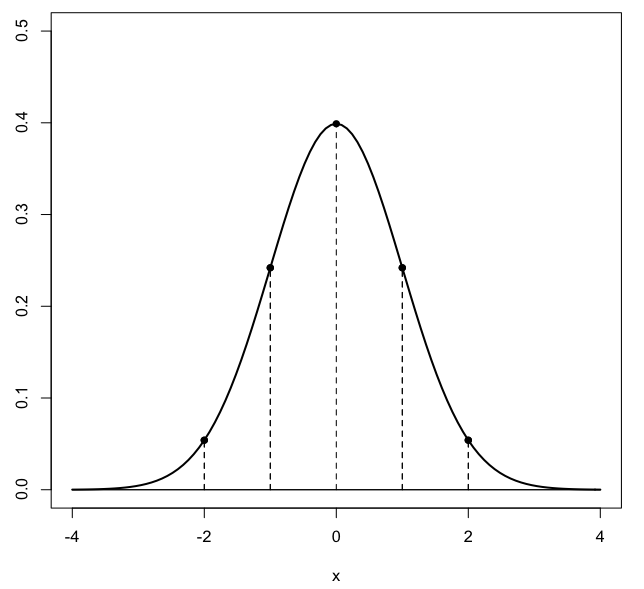
\includegraphics [scale=0.4] {gauss3.png} \end{center}
% \begin{bmatrix} a  &  b \\ c  &  d \end{bmatrix}
% \bigg |_

\begin{document}
\maketitle
\Large

This short write-up attempts to unify the vector dot and cross-products with the basic idea of a vector projection.

\subsection*{dot product}

Recall that the dot product (for vectors in n-dimensional space) can be defined to be:

\[ \mathbf{a} = \ \langle a_1,a_2, \dots a_n \rangle \]
\[ \mathbf{b} = \ \langle b_1,b_2, \dots b_n \rangle \]
\[ \mathbf{a} \cdot \mathbf{b} = a_1 b_1 + a_2 b_2 + \dots + a_n b_n \]

The dot product is the sum of the products of the individual terms
\[ = \sum_i a_i b_i \]

The dot product of two vectors is a number, in vector terminology it is called a \emph{scalar}.  The result may be positive, or negative or even zero.

The dot product of a vector with itself is the square of the length or magnitude
\[ \mathbf{a} \cdot \mathbf{a} = a_1 a_1 + a_2 a_2 + \dots \ a_n a_n \]
(this is just the extension of the Pythagorean theorem to three or more dimensions). 

We write $a = |\mathbf{a}|$, where $a$ is the length (magnitude) of $\mathbf{a}$. 

There is another definition of the dot product which can be shown to be equivalent:
\[ \mathbf{a} \cdot \mathbf{b} = |\mathbf{a}| |\mathbf{b}| \cos \theta = a b \cos \theta \]

The dot product is equal to the magnitude of $\mathbf{a}$ times the magnitude of $\mathbf{b}$ times the cosine of the angle between them.  From this definition we can see that the dot product must be independent of the coordinate system.

A proof of the second definition follows from the law of cosines.  

Involving $\cos \theta$ is particularly useful in determining when two vectors are at right angles (orthogonal) to one another---this is true if and only if the dot product is zero.

\subsection*{cross product}

Now we'll look at the cross-product.  

Suppose we have two ordinary vectors $\mathbf{u}$ and $\mathbf{v}$.  These must be in $\mathbb{R}3$ because the cross-product is only defined for vectors in $\mathbb{R}3$.

We write the cross-product as
\[ \mathbf{u} \times \mathbf{v} = \mathbf{w}  \]
The simplest definition is that the magnitude of $\mathbf{w}$ is 
\[ |\mathbf{w}| = |\mathbf{u}| |\mathbf{v}| \sin \theta \]
The symmetry with the dot product is obvious.  

The direction is defined by saying that $\mathbf{w}$ is orthogonal to the plane which contains both $\mathbf{u}$ and $\mathbf{v}$, and its sign is given by the right-hand rule.  Curl the fingers of your right hand around in the direction from $\mathbf{u}$ to $\mathbf{v}$.  Your thumb points in the direction of $\mathbf{w}$.  

The term $\sin \theta$ means that the cross-product of any vector with itself is zero.
\[ \mathbf{a} \times \mathbf{a} = \mathbf{0}  \]

To make the notation simpler, we define
\[ \mathbf{u} = \langle p,q,r \rangle \]
\[ \mathbf{v} = \langle x,y,z \rangle \]
and in order to compute the cross product, we form what looks like a really weird matrix
\[
\begin{bmatrix} 
  \hat{\mathbf{i}}  &  \hat{\mathbf{j}}  &  \hat{\mathbf{k}} \\ 
  p  &  q & r \\
  x  &  y & z
\end{bmatrix}
\]
and calculate its "determinant."
\[ \mathbf{u} \times \mathbf{v}  = (qz - ry) \ \hat{\mathbf{i}} + (rx - pz) \  \hat{\mathbf{j}}  + (py - qx) \ \hat{\mathbf{k}}  \]

We can show that this vector ($\mathbf{u} \times \mathbf{v}$) is orthogonal to the two starting vectors, $\mathbf{u}$ and $\mathbf{v}$.  Test that by forming the dot product with $\mathbf{u}$.

\[ \mathbf{u} \cdot (\mathbf{u} \times \mathbf{v})  =  p(qz - ry) + q(rx - pz)   + r(py - qx)  \] 

The first and fourth terms cancel, the second and fifth terms cancel, and the third and sixth terms also cancel.  

So $\mathbf{u} \cdot (\mathbf{u} \times \mathbf{v}) = 0$, and a similar argument shows that $\mathbf{v} \cdot (\mathbf{u} \times \mathbf{v}) = 0$ as well.  The cross-product is a convenient method to find the normal vector to a plane (defined by two vectors).

As an aside, we could have skipped this calculation.  The following rule holds for vectors:
\[ \mathbf{a} \cdot ( \mathbf{b} \times \mathbf{c} ) = ( \mathbf{a} \times \mathbf{b} ) \cdot \mathbf{c} \]

So
\[ \mathbf{u} \cdot (\mathbf{u} \times \mathbf{v}) = (\mathbf{u} \times \mathbf{u}) \cdot \mathbf{v} = 0 \cdot \mathbf{v} = 0  \]
\[ \mathbf{v} \cdot (\mathbf{u} \times \mathbf{v}) = - \mathbf{v} \cdot (\mathbf{v} \times \mathbf{u}) = - (\mathbf{v} \times \mathbf{v}) \cdot \mathbf{u} = 0 \]

\subsection*{projection}

Now, consider a standard setup with two vectors $\mathbf{a}$ and $\mathbf{b}$, which are drawn starting from the same point with an angle $\theta$ between them.  In general, the two vectors  $\mathbf{a}$ and $\mathbf{b}$ are not unit vectors.

The axes have been drawn so that  $\mathbf{a}$ is horizontal.

\begin{center} 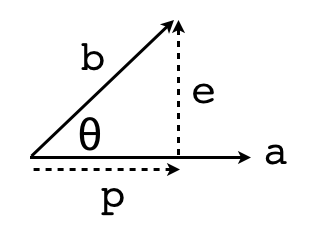
\includegraphics [scale=0.4] {dot3.png} \end{center}

We are interested in the projection of $\mathbf{b}$ on $\mathbf{a}$.  We drop a perpendicular line segment from the end of $\mathbf{b}$ onto $\mathbf{a}$.  This gives two new vectors, the projection $\mathbf{p}$ which is parallel to $\mathbf{a}$, and another vector $\mathbf{e}$ such that 

\[  \mathbf{p}  +  \mathbf{e} =  \mathbf{b} \]

Strang calls $\mathbf{e}$ the \emph{error} vector, hence the nomenclature.

How to calculate $\mathbf{p}$ and $\mathbf{e}$?  We use the fact that $\mathbf{p}$ and $\mathbf{e}$ are perpendicular.  Thus:

\[ \mathbf{p} \cdot \mathbf{e} = 0 \]

So starting from

\[  \mathbf{p}  +  \mathbf{e} =  \mathbf{b} \]
\[  \mathbf{p} \cdot \mathbf{p}  +  \mathbf{e}  \cdot \mathbf{p}  =  \mathbf{b}  \cdot \mathbf{p}  \]
\[  \mathbf{p} \cdot \mathbf{p}  =  \mathbf{b}  \cdot \mathbf{p}  \]

Here we have used the fact that the dot product is distributive over vector addition.  It is easy to show this by writing out the components.  Suppose we have three vectors $\mathbf{a}, \mathbf{b}$, and $\mathbf{c}$

\[ \mathbf{a} = \ \langle a_1,a_2, \dots a_n \rangle \]
\[ \mathbf{b} = \ \langle b_1,b_2, \dots b_n \rangle \]
\[ \mathbf{c} = \ \langle b_1,c_2, \dots c_n \rangle \]

We are to compute $\mathbf{a} \cdot (\mathbf{b} + \mathbf{c})$.

The first term of $\mathbf{b} + \mathbf{c}$ is $b_1 + c_1$, and the first term of $\mathbf{a} \cdot (\mathbf{b} + \mathbf{c})$ is of course just $a_1(b_1 + c_1) = a_1 b_1 + a_1 c_1$.  From this it is clear that $\mathbf{a} \cdot (\mathbf{b} + \mathbf{c}) = \mathbf{a} \cdot \mathbf{b} + \mathbf{a} \cdot \mathbf{c}$.

Since the projection $\mathbf{p} = t \mathbf{a}$, where $t$ is some constant, starting from what we had above

\[  \mathbf{p} \cdot \mathbf{p}  =  \mathbf{b}  \cdot \mathbf{p}  \]

we substitute using $\mathbf{p} = t \mathbf{a}$:

\[  t\mathbf{a} \cdot t\mathbf{a}  =  \mathbf{b}  \cdot t \mathbf{a}  \]

factor out one $t$

\[  t\mathbf{a} \cdot \mathbf{a}  =  \mathbf{b}  \cdot \mathbf{a}  \]
\[ t = \frac{\mathbf{b}  \cdot \mathbf{a} }{\mathbf{a}  \cdot \mathbf{a} } \]

Furthermore, if $\mathbf{a}$ has been re-scaled to be a unit vector, then $\mathbf{a}  \cdot \mathbf{a} = 1$, and this would be just $t = \mathbf{b}  \cdot \mathbf{a}$.  

Knowing $t$ we can compute $\mathbf{p} = t \mathbf{a}$ and using $\mathbf{p}$ compute also $\mathbf{e} =  \mathbf{b} - \mathbf{p}$.

Now, to come at this from another direction, recall the definition of the dot product

\[ \mathbf{a} \cdot \mathbf{b} = a b \cos \theta \] 

For simplicity, taking the case where $\mathbf{a}$ is a unit vector, we see that 

\[ \mathbf{a} \cdot \mathbf{b} = a b \cos \theta = \ b \cos \theta \]

But above we had that

\[ \mathbf{a} \cdot \mathbf{b} = t  \]

so

\[ t = \ b \cos \theta \]

and since

\[ p =  |\mathbf{p}| = |t \mathbf{a}| = t |\mathbf{a}| = t \]

It follows that

\[ p = \ b \cos \theta \]
\[ \frac{p}{b} = \cos \theta \]

And referring back to the drawing

\begin{center} 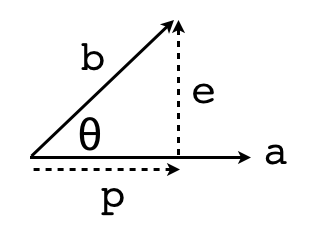
\includegraphics [scale=0.4] {dot3.png} \end{center}

\emph{of course}

\[ \cos \theta = \frac{p}{b} \]

In the same vein, 

\[ \sin \theta = \frac{e}{b} \]

So if our only concern is for the magnitude of $e$ and not its direction (suppose we are asked for the distance between the point at the end of $\mathbf{b}$ and the line defined using $\mathbf{a}$), we should recall that

\[ \mathbf{a} \times \mathbf{b} = a \ b \sin \theta = a \ b \ \frac{e}{b} = a e \]
\[ e = \frac{\mathbf{a} \times \mathbf{b}}{a} \]

The cross-product provides a way of computing $e$ without going through $\mathbf{p}$.

As a final note, it may be useful to recall that

\[ (\mathbf{a} \cdot \mathbf{b} )^2 = a^2 b^2 \cos^2 \theta \]
\[ (\mathbf{a} \times \mathbf{b} )^2 = a^2 b^2 \sin^2 \theta \]

so

\[ (\mathbf{a} \cdot \mathbf{b} )^2 + (\mathbf{a} \times \mathbf{b} )^2 = a^2 b^2 \cos^2 \theta + a^2 b^2 \sin^2 \theta \]
\[ = a^2 b^2 \]

We tie it all together by going back to the diagram again
\begin{center} 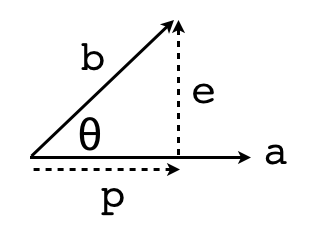
\includegraphics [scale=0.4] {dot3.png} \end{center}

\[ e = \frac{\mathbf{a} \times \mathbf{b}}{a} \]
\[ e^2 = \frac{(\mathbf{a} \times \mathbf{b})^2}{a^2} \]
\[ p^2 = b^2 \cos^2 \theta = b^2 \frac{(\mathbf{a} \cdot \mathbf{b})^2}{a^2 b^2}  =  \frac{(\mathbf{a} \cdot \mathbf{b})^2}{a^2} \]
So
\[ e^2 + p^2 =  \frac{(\mathbf{a} \times \mathbf{b})^2}{a^2} + \frac{(\mathbf{a} \cdot \mathbf{b})^2}{a^2} \]
\[ = \frac{1}{a^2} \ [ \  (\mathbf{a} \cdot \mathbf{b} )^2 + (\mathbf{a} \times \mathbf{b} )^2 \ ]  \]
\[ =  \frac{1}{a^2} \ (a^2 b^2) \]
\[ = b^2 \]

But Pythagoras already told us that.

\end{document}  